\chapter{Les lignes de transmission}

\section{Résultat numérique}
\begin{wrapfigure}[13]{l}{4.5cm}
	\vspace{-5mm}
	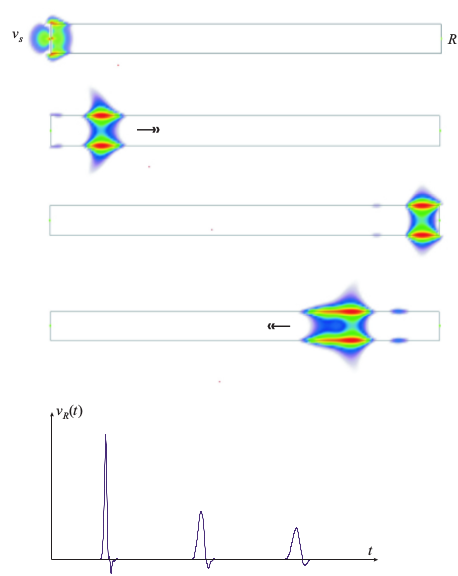
\includegraphics[scale=0.25]{ch2/image1.png}
	\captionof{figure}{ }
\end{wrapfigure}
Considérons un circuit composé uniquement d'une source de tension $s$ et d'une résistance $R$. Dans 
l'approximation quasi-statique
\begin{equation}
v_R(t) = v_s(t)
\end{equation}
Sortons de cette approximation et considérons que la tension de la source est gaussienne. Ci-dessous, 
coloré, la norme de la composante verticale du champ électrique. La ou il est non-nul, une ddp 
se crée : une \textit{onde de tension} se propage. Après $R$, une partie est \textit{réfléchie} vers 
la source. Elle peut ainsi faire plusieurs aller-retours. La \textbf{ligne de transmission} relie 
la source à la charge. Ce vocable est utilisé lorsque l'approximation quasi-statique ne s'applique 
plus. Trois types de lignes différentes sont représentées ci-dessous.
\begin{center}
	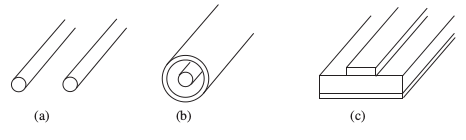
\includegraphics[scale=0.45]{ch2/image2.png}
	\captionof{figure}{(a) Ligne bifilaire (b) ligne coaxiale (c) ligne micro-ruban (microstrip). 
	Notons que l'on désigne le \textit{plan de masse} la ligne du dessous.}
\end{center}

\section{Propagation sur une ligne infinie}
La ligne infinie permet de se débarrasser des "aller-retours". Considérons une source "continue" 
de type créneau. La nouveauté est que l'on considère ici les fils : nous avons vu que la ddp entre 
ceux-ci dépend de la position et du temps : $v=v(z,t)$.\\
Considérons une source idéale $v_s$. Avant enclenchement, la ligne est neutre. Une fois celle-ci 
allumée, sous l'effet d'un champ électrique, il apparaît des densités de charges induites 
créant une ddp $v_s$. Ces charges induites provoquent l'apparition d'un champ électrique un peu 
plus loin sur la ligne : ce dernier se propage sans être atténué. Le signal n'est donc pas donné 
par le mouvement des $e^-$ (qui eux sont "plaqués" à l'extérieur de la ligne) mais par le déplacement 
du champ électrique. La ligne sert ainsi de \textit{guide} pour le champ électrique par apparition 
de charges induites.\newpage


\begin{wrapfigure}[14]{l}{5.5cm}
%	\vspace{-5mm}
	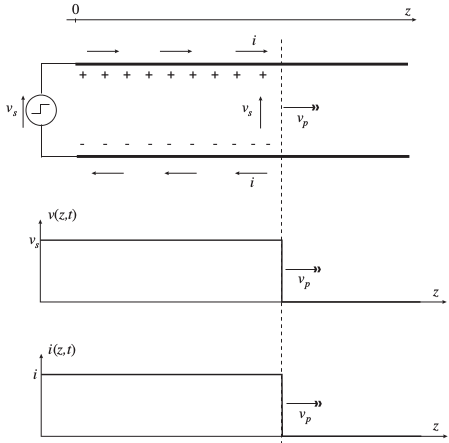
\includegraphics[scale=0.35]{ch2/image3.png}
	\captionof{figure}{ }
\end{wrapfigure}
Cette ddp $v(z,t)$ est liée à la densité de charge induite $q_l(z,t)$ par la capacité linéique de 
la ligne $C_1$
\begin{equation}
v(z,t) = \dfrac{q_l(z,t)}{C_1}
\label{eq:LienCapa}
\end{equation}
En tenant compte du délai de propagation
\begin{equation}
v(z,t) = v_s(t-z/v_p)
\end{equation}
où $v_s$ est la vitesse de propagation (inconnue). On en tire
\begin{equation}
\dfrac{\partial v}{\partial z} = -\dfrac{1}{v_p}\dfrac{\partial v}{\partial t}
\label{eq:ASat}
\end{equation}
La densité de charge induite est nulle lorsque 
le font d'onde n'est pas passé et vaut $v_sC_1$ la ou il est déjà passé : la ligne se charge. La 
ou le front d'onde est passé, les $e^-$ ont subi un déplacement microscopique formant un champ qui 
lui même, crée un courant : \textit{onde de courant}. Celle-ci doit satisfaire
\begin{equation}
\dfrac{\partial i}{\partial z} = -\dfrac{1}{v_p}\dfrac{\partial i}{\partial t}
\end{equation}
Avec cette relation et la conservation de la charge $\displaystyle\dfrac{\partial i}{\partial z} 
=-\dfrac{\partial q_l}{\partial t}$ on obtient après intégration (charge initiale et courant 
initial nuls $\forall z$)
\begin{equation}
i(z,t) = v_pq_l(z,t)
\end{equation}
En utilisant cette relation de \autoref{eq:LienCapa} on remarque que le rapport tension/courant 
est constant en tout point de la ligne\footnote{Pour une onde de tension/courant donnée.}
\begin{equation}
\dfrac{v(z,t)}{i(z,t)} = \dfrac{1}{v_pC_1}\triangleq Z_C
\label{eq:DefZC}
\end{equation}
où $Z_C$ est l'\textbf{impédance caractéristique} de la ligne : vraie pour la source en $z=0$ et 
équivalente pour la ligne infinie à une résistance de cette valeur : la ligne absorbe en 
permanence un courant $v_s/Z_c$.


\section{Les équations des lignes}
\begin{wrapfigure}[6]{r}{7.5cm}
	\vspace{-5mm}
	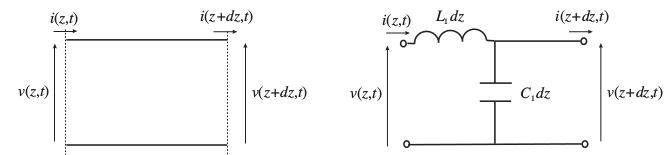
\includegraphics[scale=0.35]{ch2/image4.png}
	\captionof{figure}{ }
\end{wrapfigure}
Il faut procéder à une décomposition infinitésimale car pas d'effet de retard. Considérons 
un tel tronçon. On peut voir un tel tronçon comme une capacité valant $C_1dz$. Comme un courant 
génère un $\vec{B}$, le tronçon captera un flux : apparition d'une inductance par unité de 
longueur
\begin{equation}
L_1 = \dfrac{\phi_1}{i}
\end{equation}
Comme le tronçon est infinitésimal, la théorie des circuit s'applique. Le circuit équivalent 
peut s'écrire mathématiquement
\begin{equation}
\begin{array}{ll}
v(z+dz,t) &= v(z,t) - L_1dz\dfrac{\partial i(z,t)}{\partial t}\\
i(z+dz,t) &= i(z,t) - C_1dz\dfrac{\partial v(z,t)}{\partial t}
\end{array}
\end{equation}
où encore\\

\retenir{\ \textbf{équations des télégraphistes}.
\begin{equation}
\begin{array}{ll}
\dfrac{\partial v(z,t)}{\partial z} &= -L_1 \dfrac{\partial i(z,t)}{\partial t}\\
\dfrac{\partial i(z,t)}{\partial z} &= -C_1 \dfrac{\partial v(z,t)}{\partial t}
\end{array}
\label{eq:Telegraphistes}
\end{equation}}\ 

Ces équations montre que le courant correspond au courant injecté, diminué du courant de 
fuite dans les capacités. En découplant le système (remplace l'une dans l'autre après 
en avoir dérivée une) en augmentant l'ordre, on retrouve les équations d'ondes
\begin{equation}
\begin{array}{ll}
\dfrac{\partial^2 v(z,t)}{\partial z^2} &= L_1C_1\dfrac{\partial^2 v(z,t)}{\partial t^2}\\
\dfrac{\partial^2 i(z,t)}{\partial z^2} &= L_1C_1\dfrac{\partial^2 i(z,t)}{\partial t^2}
\end{array}
\end{equation}
Les tensions et courants se propagent donc à la vitesse 
\begin{equation}
v_p = \dfrac{1}{\sqrt{L_1C_1}}
\end{equation}
On peut écrire, à partir de la définition \autoref{eq:DefZC} de $Z_C$\\
\retenir{\begin{equation}
Z_C = \sqrt{\dfrac{L_1}{C_1}}
\end{equation}}
La solution de ces équations est bien connues : il s'agit d'ondes progressives (droite) ou 
régressives (gauche) se déplaçant à vitesse constante. Le premier type de solution à la 
forme
\begin{equation}
v_+(z,t) = V_+f(t-z/v_p)\qquad V_+\in\mathbb{R}
\end{equation}
où $f$ est une fonction quelconque. Cette solution satisfaisant \autoref{eq:ASat} correspond 
à une tension se propageant le long de la ligne sans atténuation ni déformation. Pour trouver 
le courant $i_+(z,t)$ associé, on utilise
\begin{equation}
\left\{\begin{array}{l}
\autoref{eq:ASat}\\
\autoref{eq:Telegraphistes}
\end{array}\right.\quad\Longrightarrow\quad \dfrac{\partial i_+(z,t)}{\partial t} = 
\dfrac{1}{v_pL_1}\dfrac{\partial v_+(z,t)}{\partial t}
\end{equation}
Après intégration
\begin{equation}
i_+(z,t) = \dfrac{v_+(z,t)}{Z_c}
\end{equation}
Le second type de solution (régressive) est de la forme
\begin{equation}
v_+(z,t) = V_-g(t+z/v_p)\qquad V_-\in\mathbb{R}
\end{equation}




On peut déduire le courant $i_-(z,t)$ (conventionnellement choisi opposé à $i(z,t)$, 
le courant étant défini positif de gauche à droite sur la ligne supérieur) associé à 
cette onde par résolution de l'ED suivante (similairement au cas de l'onde progressive)
\begin{equation}
\dfrac{\partial i_(z,t)}{\partial t} = -
\dfrac{\partial i(z,t)}{\partial t} = \dfrac{1}{v_pL_1}\dfrac{\partial v_-(z,t)}{\partial t}
\end{equation}
Après intégration
























